\section{Metodologia}\label{sec-metodologia}

As revisões sistemáticas da literatura representam abordagens
metodológicas que buscam identificar, avaliar e interpretar tendências
em um dado campo de estudo \cite{Garcia-Penalvo2022}. Por se tratar de uma
proposta conceitual transdisciplinar emergente, a consideramos a mais
adequada para delinear o debate sobre literacia algorítmica (LA) nesta
investigação. Projetadas para reduzir vieses e fornecer evidências para
embasar debates acadêmicos, a revisão sistemática de literatura envolve
uma série de passos, como introdução, planejamento, realização e relato
da revisão \cite{White2005}. Neste artigo, estruturamos cada etapa
a partir de quatro questões \Cref{tab-01}. A definição das questões de
pesquisa é a etapa mais importante de uma revisão sistemática de
literatura, pois estabelece as bases que orientam as decisões ao longo
do processo de investigação, buscando, assim, efetivamente contribuir
para a produção de conhecimento sobre lacunas em uma dada literatura
\cite{Garcia-Penalvo2022}.

Em nosso estudo, as questões são construídas a partir de quatro eixos de
investigação sobre a ideia de literacia algorítmica: a) suas propostas
conceituais, b) as técnicas e as estratégias pedagógicas emergentes
nestes debates, c) funções e espaços de aplicação destes conhecimentos
e, por fim, d) os desafios e as dificuldades retratadas na literatura. A
partir destes eixos, identificamos quatro questões norteadoras da
revisão, apresentadas no \Cref{tab-01}.

\begin{table}[!htpb]
\centering
\begin{threeparttable}
\caption{Questões orientadoras do processo de revisão
sistemática de literatura sobre literacia algorítmica}
\label{tab-01}
\begin{tabular}{p{0.97\textwidth}}
\toprule
Q1: Quais são os modelos conceituais que compõem a literacia algorítmica
e como estas propostas se diferem de outras formas de literacia, como a
digital ou a midiática? \\
Q2: Quais são as abordagens pedagógicas relacionadas à literacia
algorítmica e como elas funcionam na promoção de conhecimento e
consciência sobre a ação de algoritmos? \\
Q3: Quais são as principais atividades ou áreas de conhecimento em que a
literacia algorítmica é aplicada? \\
Q4: Quais são os principais obstáculos enfrentados no desenvolvimento da
literacia algorítmica, considerando os diferentes fatores como educação,
acesso à tecnologia e cultura digital? \\
\bottomrule
\end{tabular}
\source{Elaboração própria.}
\end{threeparttable}
\end{table}
    
O processo de seleção das publicações analisadas neste artigo foi
inspirado pela chamada declaração PRISMA \cite{Moher2009},
que se configura como um fluxo de análise com quatro fases para revisões
sistemáticas. Em nossa investigação, nos apropriamos das primeiras três
etapas da declaração PRISMA (identificação, triagem e elegibilidade),
por considerar que dão conta do processo de qualificação da seleção de
publicações a serem analisadas e da redução de vieses.

A \Cref{image-01} apresenta o fluxo de seleção das publicações analisadas nesta
revisão sistemática sobre LA. Na Fase 1, Identificação, momento de
captação inicial das publicações, utilizamos duas importantes bases de
dados, a Scopus e a Web of Science. A escolha delas foi fundamentada na
abrangência e na reputação acadêmica. Ambas as plataformas são
conhecidas por indexarem um amplo espectro de revistas científicas,
conferências e outras fontes relevantes, garantindo uma busca abrangente
e diversificada de publicações sobre o tema. Além disso, a Scopus e a
Web of Science possuem recursos avançados de filtragem e busca,
permitindo a utilização de descritores específicos em múltiplos idiomas,
como português, inglês e espanhol, o que possibilitou uma abordagem
multilíngue na captação de artigos e pesquisas relacionadas à LA. A
busca foi conduzida utilizando termos nos três idiomas. Em português e
espanhol, acionamos os descritores `Literacia AND Algorítmica'. Já para
a língua inglesa, usamos os descritores `\emph{algorithmic OR algorithm
AND literacy OR literacies}'. No sistema de busca das duas plataformas,
os termos foram pesquisados no título, resumo e palavras-chave das
publicações. Ao final do processo de busca, identificamos um total de 42
publicações na Scopus e 25 na Web of Science.

\begin{figure}[h!]
\centering
\begin{minipage}{0.85\textwidth}
\caption{Fluxo de seleção das publicações a serem analisadas.}
\label{image-01}
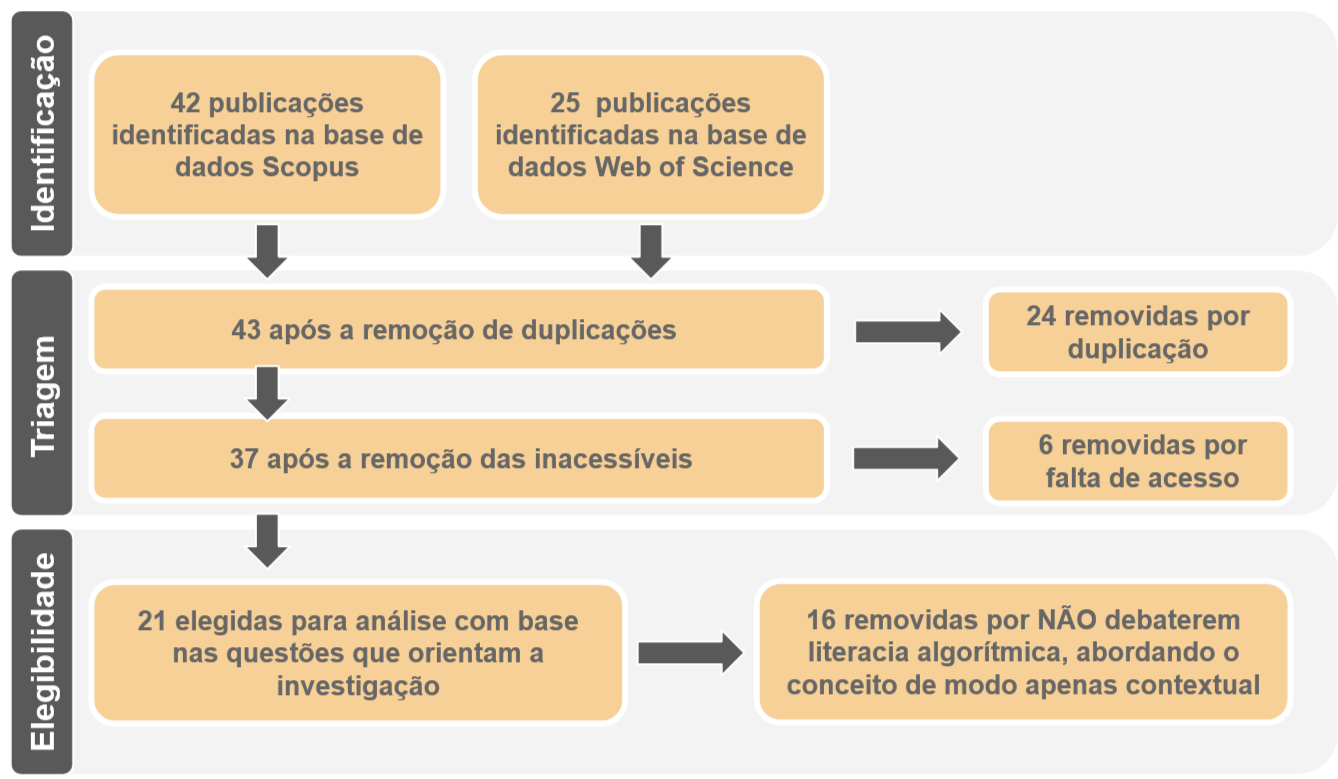
\includegraphics[width=\linewidth]{image1.png}
\source{Elaboração própria.}
\end{minipage}
\end{figure}

Na fase de Triagem, foram identificadas 24 publicações duplicadas, ou
seja, estudos que apareceram em ambas as plataformas de busca. Ademais,
durante a triagem, 6 publicações foram consideradas inacessíveis pelos
pesquisadores. Esses trabalhos não puderam ser obtidos por diferentes
motivos: restrições de assinatura, pagamento em determinadas plataformas
ou indisponibilização do texto completo pelos autores ou revistas. A
decisão de remover essas publicações inacessíveis foi tomada com base na
necessidade de garantir a confiabilidade e a completude da revisão,
visto que a impossibilidade de acessar o conteúdo completo poderia
afetar negativamente a análise e a interpretação dos resultados.

Após identificação e remoção das duplicações e publicações inacessíveis,
restaram 37 artigos para a fase de Elegibilidade. Nessa etapa, tornam-se
fundamentais os critérios de inclusão e exclusão. Tais definições são
estabelecidas para garantir que o foco analítico das questões
orientadoras se reflita na seleção das publicações, dando maior clareza
e eficiência ao processo de análise. Conforme mostra a \Cref{tab-02}, os
critérios de inclusão contemplam estudos que abordam o conceito de LA,
apresentam propostas e reflexões sobre práticas para geração de
literacia algorítmica, além de artigos escritos em português, inglês ou
espanhol publicados até a data do corte desta revisão (dezembro de
2022). Já os critérios de exclusão buscam eliminar estudos cujo texto
completo estava indisponível no momento da coleta de dados, trabalhos
não relacionados à LA e estudos em que a LA é abordada apenas como
elemento contextual para análise de uma temática mais específica.

   
\begin{table}[!htpb]
\centering
\begin{threeparttable}
\caption{Critérios de seleção para fase de elegibilidade}
\label{tab-02}
\begin{tabular}{p{0.475\textwidth} p{0.475\textwidth}}
\toprule
Critérios de Inclusão & Critérios de Exclusão \\
\midrule
Estudos que abordam o conceito de literacia algorítmica. & Estudos que não estavam com o texto completo à disposição dos pesquisadores no momento da captação de dados.\\
Estudos que apresentam propostas e reflexões sobre práticas para geração de literacia algorítmica. & Estudos que não estejam relacionados à literacia algorítmica;\\
Artigos escritos em português, inglês ou espanhol. & Estudos nos quais literacia algorítmica é acionada apenas como elemento contextual para análise de uma temática mais específica. \\
Publicações disponíveis até a data do corte desta revisão (dezembro de 2022). & \\
\bottomrule
\end{tabular}
\source{Elaboração própria.}
\end{threeparttable}
\end{table}   


Na etapa de Elegibilidade, o processo de análise consistiu em uma
leitura minuciosa dos textos das publicações, junto à produção de
resumos sobre cada pesquisa e seus principais achados. A partir desses
resumos e dos textos originais, a análise de elegibilidade foi
conduzida. O critério de exclusão com maior preponderância foi a
eliminação de publicações que não aprofundam a discussão sobre o
conceito de literacia algorítmica ou não apresentam propostas formativas
ou pedagógicas relacionadas ao tema (ao todo, 16). Nessas publicações, a
literacia algorítmica surge como discussão lateral, geralmente acionada
como um imperativo para a educação contemporânea, sem explorar de forma
substancial seu significado ou suas possíveis aplicações. Podemos citar
o artigo de \textcite[p.~759]{Cotter2020}, que analisa como o
contexto socioeconômico segue moldando o uso de tecnologias digitais e
aprofundando disparidades, o que indica que ``uma maior literacia
algorítmica também pode implicar na familiaridade com o funcionamento
dos algoritmos, bem como na habilidade de avaliar seus resultados
informativos''. Embora destaquem a relevância da literacia algorítmica,
não há um debate sobre o que exatamente compreende este conceito. De
modo similar, o artigo de \textcite{Kapsch2022}, que explora como jovens adultos
dão sentido e refletem sobre sua agência enquanto usuários em relação
aos algoritmos, enxerga a literacia algorítmica como um possível
resultado da proposta metodológica do estudo, sem efetivamente traçar
uma definição sistemática. Ainda neste grupo de trabalhos eliminados na
fase de Elegibilidade, há uma série de estudos que posicionam a
literacia algorítmica como ferramenta da aprendizagem de matemática e
computação \cite{Astambayeva2021,How2022}, abordagem que
se distancia dos objetivos e questões orientadoras de nosso estudo.
